%----------------------------------------------------------------------------------------
%	PACKAGES AND OTHER DOCUMENT CONFIGURATIONS
%----------------------------------------------------------------------------------------

\documentclass[paper=a4, fontsize=11pt, oneside]{scrartcl} % A4 paper and 11pt font size

\usepackage[T1]{fontenc} % Use 8-bit encoding that has 256 glyphs
\usepackage{fourier} % Use the Adobe Utopia font for the document - comment this line to return to the LaTeX default
\usepackage[english]{babel} % English language/hyphenation
\usepackage{amsmath,amsfonts,amsthm} % Math packages

\usepackage{lipsum} % Used for inserting dummy 'Lorem ipsum' text into the template

\usepackage{sectsty} % Allows customizing section commands
\allsectionsfont{\centering \normalfont\scshape} % Make all sections centered, the default font and small caps

\usepackage{rotating} % Used for sidewaysfigure and other rotation options.

\usepackage[parfill]{parskip}

\usepackage{fancyhdr} % Custom headers and footers
\pagestyle{fancyplain} % Makes all pages in the document conform to the custom headers and footers
\fancyhead{} % No page header - if you want one, create it in the same way as the footers below
\fancyfoot[L]{} % Empty left footer
\fancyfoot[C]{} % Empty center footer
\fancyfoot[R]{\thepage} % Page numbering for right footer
\renewcommand{\headrulewidth}{0pt} % Remove header underlines
\renewcommand{\footrulewidth}{0pt} % Remove footer underlines
\setlength{\headheight}{13.6pt} % Customize the height of the header

\usepackage{graphicx} % Allows the use of images in the document
\graphicspath{ {images/} } % Instructs LaTeX to search the 'images' directory for images.

%\numberwithin{equation}{section} % Number equations within sections (i.e. 1.1, 1.2, 2.1, 2.2 instead of 1, 2, 3, 4)
%\numberwithin{figure}{section} % Number figures within sections (i.e. 1.1, 1.2, 2.1, 2.2 instead of 1, 2, 3, 4)
%\numberwithin{table}{section} % Number tables within sections (i.e. 1.1, 1.2, 2.1, 2.2 instead of 1, 2, 3, 4)

%\setlength\parindent{0pt} % Removes all indentation from paragraphs - comment this line for an assignment with lots of text

%----------------------------------------------------------------------------------------
%	TITLE SECTION
%----------------------------------------------------------------------------------------

\newcommand{\horrule}[1]{\rule{\linewidth}{#1}} % Create horizontal rule command with 1 argument of height

\title{	
\normalfont \normalsize 
\textsc{Concordia University} \\
\textsc{Department of Computer Science and Software Engineering} \\
\textsc{SOEN 341/4 S \qquad Software Process \qquad Winter 2016} % University, school and/or department name(s)
\horrule{0.5pt} \\[0.4cm] % Thin top horizontal rule
\huge Mytinerary: \\ System Overview and Team Members \\ % The assignment title
\horrule{2pt} \\[0.5cm] % Thick bottom horizontal rule
}

\author{Team AnotherOne} % Names

\date{\normalsize January 13, 2016} % Date

\begin{document}

\maketitle % Print the title

%----------------------------------------------------------------------------------------
%	SYSTEM OVERVIEW
%----------------------------------------------------------------------------------------

\section*{System Overview}
This document presents an initial outline of Mytinerary, a web application designed to adjust and optimize the schedules of Concordia Software Engineering students.

The system will be used to generate a list of possible multi-semester schedules for a Concordia student. Each schedule will be constrained by the requirements that 1) it satisfies the preferences the user selected; 2) the schedule meets the user's program requirements; and 3) every course is taken after any prerequisites or concurrently with any co-requisites. Examples of possible user preferences include (but are not limited to) preferred course load, available times, and desired graduation date.

Mytinerary contains only two user classes: the student, who can set their preferences and request schedules; and the program director, who can view and edit the academic record of any student in their respective program, and can modify course section details.

\begin{figure}[H]
\centering
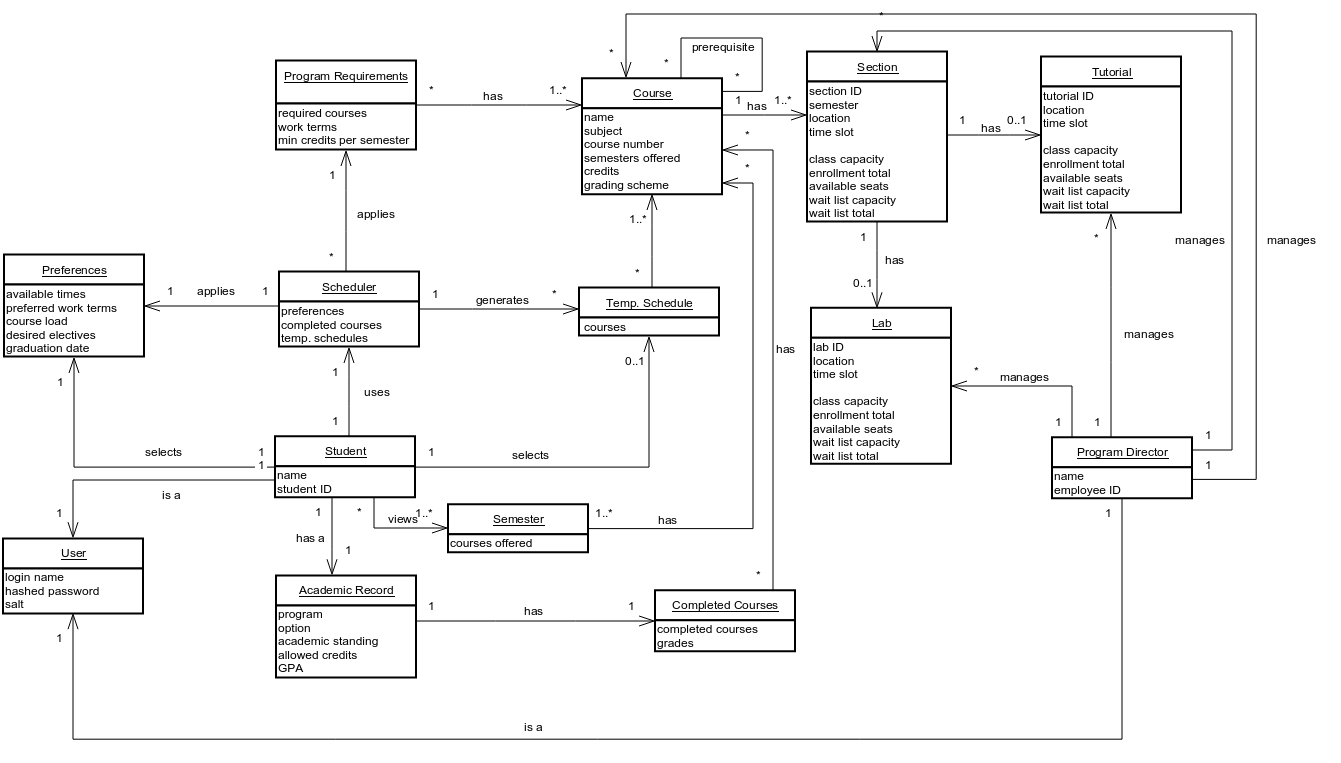
\includegraphics[width=1.4\textwidth, angle=-90]{domain_model}
\caption{Domain Model for the Mytinerary scheduling system}
\label{fig:domain_model}
\end{figure}

Figure \ref{fig:domain_model} illustrates a domain model for our system. The principal domain objects are the student, the course section, and the scheduler itself. Students, who are users, have preferences and an academic record and interact with the scheduler. The scheduler in turn consults the student's academic record and preferences, the requirements of the program the student is enrolled in, and the available course sections offered in each semester to generate a list of tentative schedules for the student to select. Course sections consist possibly of a tutorial section and a lab and are in turn instances of the more general course object. Finally there are program directors, who are users of the system with the privilege to view and modify a student's academic record and manage course details.

%----------------------------------------------------------------------------------------
%	TEAM MEMBERS
%----------------------------------------------------------------------------------------
\section*{Team Members}



\end{document}